%        File: brainiak_writeup.tex
%     Created: Fri Sep 28 10:00 AM 2018 E
% Last Change: Fri Sep 28 10:00 AM 2018 E
%
\documentclass[a4paper]{article}

\usepackage{graphicx}
\usepackage{amsmath}
\usepackage[linesnumbered,ruled]{algorithm2e}

\title
{Model Based Inter-Subject Correlations with Latent Time Series}
\author{Nathan Wycoff}

\begin{document}
\maketitle

\section{Introduction}

When presenting a fMRI subject with a stimulus, the volume of noise inherent in a human brain make it difficult to extricate which dynamics are effects of the experiment, and which are due to extrinsic factors. One approach to resolve the signal to noise problem is Inter-Subject Correlations (ISC), which conjectures that, given $N$ many subjects, each exposed to the same stimulus over the same time course, correlations between subjects ought to be due to the stimulus as opposed to due to extrinsic factors. For this reason, calculating which regions of the brain share characteristics is of great interest in fMRI studies. Existing methods to calculate ISC are based on heuristics. In this article, we present a model based approach to ISC calculation, developed during the 2018 VTCRI Brainihak Hackathon. As the product of a Hackathon, the approach has only just been briefly explored. In the conclusion, we present paths for future work.

\section{Heuristic ISC Calculation}

The existing method for ISC calculation involves determining the correlation between each subject and the mean of all other subjects iteratively for each voxel, as shown in Algorithm \ref{heurisc}.

\begin{algorithm}
    \label{heurisc}
    \SetKwInOut{Input}{Input}
    \SetKwInOut{Output}{Output}

    \underline{function heur\_isc} $(\mathbf{Y})$\;
    \Input{$\mathbf{Y}$ - Tensor of voxel by time by subject observations, $\mathbf{Y} \in \mathbb{R}^{V \times T\times N}$}
    \Output{Correlations / p values}

    \For{$v\gets1$ \KwTo $V$}{
        \For{$i\gets1$ \KwTo $N$}{
            $r_{v,i} \gets \textrm{cor}(Y_{v,i,.}, \bar Y_{v,-i,.})$
        }
        $r_{v,.} \gets \textrm{mean}(r_{v,i})$
    }
    \caption{Heuristic ISC}
\end{algorithm}

\section{A Generative Time-Series Approach }

Generally, modeling means is more intuitive than modeling complicated covariances. One way to induce complex dependence structures is to assume the existence a latent mean structure which is then marginalized out. This is the approach this article takes. Fix some voxel $v$ that is responsible for reacting to the stimulus. Our model assumes that there exists some unobserved mean value for this voxel shared across all participants that follows an Auto-Regressive process. The generative model is shown in Algorithm \ref{generative}. $Z_{v,t}$ is the latent voxel intensity for voxel $v$ at time $t$, $Y_{v,t,i}$ gives the observed value at voxel $v$, time $t$ of subject $i$. $\phi$ is the AR coefficient, and $\sigma_{z,v}$ and $\sigma_{y,v}$ are error variances for the latent processes and the observed values. The model assumes a different variance for each voxel, though the stronger assumption of shared variances may also be made.

\begin{algorithm}
    \label{generative}
    \SetKwInOut{Input}{Input}
    \SetKwInOut{Output}{Output}

    \underline{function lts\_gen} $(\mathbf{Y})$\;
    \Input{$V$ - Number of Voxels \newline
    $T$ Number of Timepoints\newline
    $N$ Number of Participants}
    \Output{Correlations / p values}

    \For{$v\gets1$ \KwTo $V$}{
        $Z_{v,1} \sim N(0, \sigma_{z,v})$

        \For{$t\gets2$ \KwTo $T$}{
            $Z_{v,t} \sim N(\phi_v Z_{v,t-1}, \sigma_{z,v})$
        }
    }
    \For{$i\gets1$ \KwTo $N$}{
        \For{$v\gets1$ \KwTo $V$}{
            \For{$t\gets2$ \KwTo $T$}{
                $\mathbf{Y}_{v,t,i} \sim N( Z_{v,t}, \sigma_{y,v})$
            }
        }
    }
    \caption{The LTS generative model.}
\end{algorithm}

For voxels which are not active, we simply assume a normal distribution. For simplicity, the data are assumed to be mean zero. When applying this model to real data, it will be important to include a mean term in the model. This will not generally cause much additional complication.

The central inference question is now, given $\mathbf{Y}$, to determine which voxels are drawn from the active distribution, and which from the inactive distribution. This may be framed as a statistical model selection problem. The process is simplified by noting that our models are nested: if $\phi_v = \sigma_{z,v} = 0$, then $Z_{v,t} = 0 \forall t$, giving a mean zero variance $\sigma_{{y,v}^2}$  distribution on $Y_{v,t,i} \forall t,i$, exactly our null distribution. Phrasing our model as a problem of this form allows us to bring to bear much of the nested model selection research that has occurred in the statistics community over the past half century. 

Two central approaches come to mind: Likelihood Ratios (LR) and Bayes Factors (BF) (though penalization type approaches such as LASSO could also be considered). During the Hackathon, we developed a likelihood ratio approach which could easily be converted into asymptotic p-values. 

Before calculating either LR or BF, it is necessary to integrate out the nuisance parameters $Z$. Fortunately, due to the reproducibility property of the Gaussian, such an integral may be carried out analytically, giving (what I think at this point is) a Matrix Normal distribution on $\mathbf{Y}_{v,.,.}$:

$$
P(\mathbf{Y}_{v,.,.} | \Sigma, \sigma_{y,v}) = 
|\frac{4 \pi^2}{\sigma^2}\Sigma \Sigma_z|^{-1/2}
e^{-0.5[\frac{\textrm{tr}(Y'Y)}{\sigma^2_{y,v}} - \mu_z'\Sigma_z^{-1}\mu_z]}
$$

This likelihood on $\mathbf{Y}$ is (based on initial numerical experiments) convex in $\phi, \sigma_{y,v}$ and $\sigma_{z,v}$, leading to easy inference on model parameters, and thus LR calculation.

For calculation of BF, it is also necessary to integrate out the other model parameters. I have not attempted this, but would guess that integrating out one or two of these analytically is possible, leading to a 1 or 2D integral to be easily solved via quadrature.

AR processes automaticall induce a covariance matrix on $Z_{v,}$, call it $\Sigma$, a function of $\sigma_{z,v}$ and $\phi_v$. Let $\Sigma_z = (\frac{1}{\sigma^2} \mathbf{I} + \Sigma^{-1})^{-1}$ and $\mu_z = (\Sigma_z)(\frac{\sum_{i=1}{N}\mathbf{Y}_{v,i,.}}{\sigma^2})$.

\section{Results and Perspectives}

To verify feasibility of the approach, we generated data from Algorithm \ref{generative}, and plotted a RoC curve of the LTS versus the heuristic approach. They appear to have comparable performance for most simulations, such as the one in Figure \ref{fig:roc}. However, there is much room for improvement. 

Let's discuss future work. Bayes Factors would likely yield better results than the LR attempted here. There are also many choices for the latent mean besides an AR model that could be explored. The implementations are written in python with minimal care to numerical accuracy and speed: considerable speedups are possible if matrix inversion and determinant calculation would take the special structure of our covariance matrix into account. All this work was done under the extreme time constraints of a 48-hour event: there is much room to develop a powerful model based approach.

\begin{figure}[h]
    \centering
    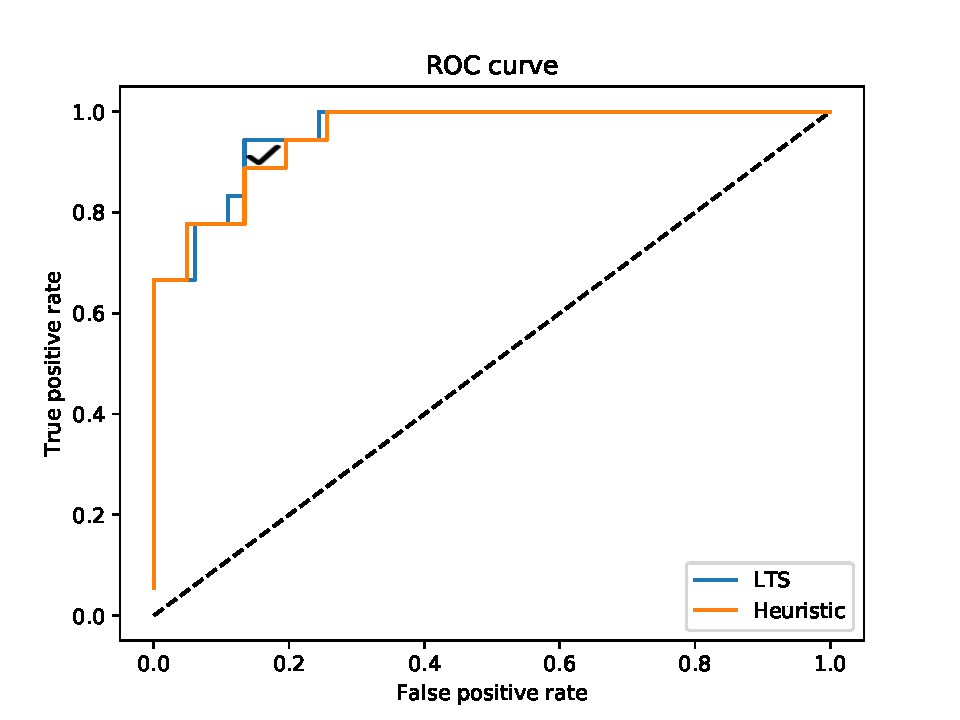
\includegraphics[scale=0.8]{../images/roc.pdf}
    \caption{The ROC curve for the competing approaches with $V = 100$, $N = 30$, $T = 100$.}
    \label{fig:roc}
\end{figure}

\end{document}
